%----------------------------------------------------------------------------------------
%	SECTION 1.1
%----------------------------------------------------------------------------------------

\section{The Channel Coding Theorem.}
\label{section1}

We begin this section with two results.

\begin{lemma}\label{3.2.1}
    For any discrete memoryless channel, with capacity $C_{\max}$, the DMC can
    transmit at most $C_{\max}$ bits of information per unit time.
\end{lemma}
\begin{corollary}
    If $X$ is a test source achieving  $C(\beta_{\max})=C_{\max}$, then the DMC
    can transmit at leeast $C_{\max}$ bits of information per unit time.
\end{corollary}
\begin{remark}
    So, if we choose our test source right, we can transmit, with the DMC,
    exactly $C_{\max}$ bits of information per unit time; i.e. we transmit all
    communcations optimally at channel capacity.
\end{remark}

\begin{definition}
    We define the \textbf{rate} of a channel to be the ratio
    \begin{equation}
        \frac{k}{n}
    \end{equation}
    of number of symbols transmitted per channel use.
\end{definition}

\begin{lemma}\label{3.2.2}
    Given a channel with rate $\frac{k}{n}$, and $\epsilon>0$ small enough, such
    that for input and output sequences  $\{U_i\}$ and $\{\hat{U}_i\}$,
    respectively, $P(\hat{U}_i \neq U_i)<\epsilon$, then:
    \begin{equation}
        \frac{k}{n} \leq \frac{C(\beta)}{1-H(\epsilon)}
    \end{equation}
\end{lemma}
\begin{proof}
    Let $U=\{U_i\}_{i=1}^k$ be a sequence of independent random variable with
    distribution $P(U=0)=P(U=1)=\frac{1}{2}$. Let $X=(X_1, \dots, X_n)$ and $Y=(Y_1,
    \dots, Y_n)$ be channel inputs and outputs respectively, with $X$ an encoding of
     $U$. Now, from  $Y$ decode the recieved message as  $\hat{U}=(\hat{U}_1, \dots,
    \hat{U}_k)$.

    Suppose $P(\hat{U}_i)<\epsilon$ for $1 \leq i \leq k$ and  $\epsilon>0$ small
    enough. Then  $I(U,\hat{U}) \geq \sum_{i=1}^k{I(U_i,
    \hat{U}_i)}=\sum{H(U_i)-H(U_i|\hat{U}_i)}=\sum{\log{2}-H(U_i|\hat{U}_i)} \geq
    \log{2}-H(\epsilon)$ by theorem \ref{2.2.2} and Fano's inequality. So
    $I(U,\hat{U}) \geq k-kH(\epsilon)$ Then, by the data processing theorem, we
    have:
    \begin{equation*}
        I(U,\hat{U}) \leq I(X,Y) \leq C_n(\beta)=nC(\beta)
    \end{equation*}
    thus we get,
    \begin{equation*}
        \frac{k}{n} \leq \frac{C(\beta)}{1-H(\epsilon)}
    \end{equation*}
\end{proof}
\begin{remark}
    What this says is that we cannot cimmunicate above the channel capacity
    $C_{\max}$.
\end{remark}

We come now to the next big definition of information theory.

\begin{definition}
    Let $n \in \Z^+$ and let  $D=(A_X,A_Y,Q)$ be a discrete memoryless cahnnel.
    We define a \textbf{channel code} of \textbf{length} $n$ to be a subset $\Cc
    \subseteq A_X^n$ with $\Cc=\{x_1, \dots x_M\}$ for some $M \in \Z^+$. We
    call the elements of  $\Cc$  \textbf{codewords}.

    We define the \textbf{rate} of the code $\Cc$ to be :
    \begin{equation}
        R=\frac{1}{n}\log{M}
    \end{equation}
    We say that $\Cc$ is  \textbf{$\beta$-admissible} of
    $b(x_i)=\sum_{j}{b(x_{ij})} \leq n\beta$ for all $i$ and  $\beta>\beta_0$.

    We define a  \textbf{decoding rule} for the code $\Cc$ to be a map  $f:A_Y^n
    \rightarrow \Cc \cup \{e\}$, where $e$ is called the \textbf{error}. We
    define an \textbf{encoding rule} to be a $1-1$ map from all possible source
    sequences into $\Cc$.

    We define the \textbf{error probability} of transmitting the codeword $x_i$
    of $\Cc$ to be:
    \begin{equation}
        P_e^{(i)}=P(f(y) \neq x_i)=\sum_{f(y) \neq x_i}{p(y|x_i)}
    \end{equation}
    where $p(y|x_i)=\prod_{j=1}^n{p(y_i|x_{ij})}$ is the product of all
    transitional probabilities of $D$, i.e. the product of all the entries of
    $Q$.
\end{definition}
\begin{remark}
    Here, we take the codeword $x$ to be an encoding of the message $u$ which
    we regard as already having been transmitted.
\end{remark}

\begin{example}
    \begin{enumerate}
        \item[(1)] Consider the binary symmetric channe (BSC) wiht
            $b(0)=b(1)=0$. For $n=3$,  $M=2$, define the code  $\Cc \subseteq
            \F_2^3$ by  $\Cc=\{(000),(111)\}$. The rate for the code is
            $R=\frac{1}{3}\log{2}=\frac{1}{3}$.

            Now, define the decoding rule $f:y_1y_2y_3 \rightarrow xxx$ such
            that $x=y_1$ if $y_1=y_2$ and $y_1=y_3$, $x=y_2$ if $y_2=y_1$ or
            $y_2=y_3$ and $x=y_3$ if  $y_3=y_1$ or $y_3=y_2$; i.e. we take the
            majority vote on the three bits. Then
            $P_e^{(1)}=P_e^{(2)}=3p^2-2p^3<p<\frac{1}{2}$.

        \item[(2)] Consider the DMC defined in example $3.1(2)$, with
            $b(0)=b(1)=1$ and $b(\frac{1}{2})=0$. Take $e=\frac{1}{2}$ to be the
            error. Define the code $\Cc \subeteq A_X^n$ by  $\Cc=\{(x_1, \dots,
            x_k, \frac{1}{2}, \dots, \frac{1}{2}) : x_i \in \F_2 \text{ and } 1
            \leq i \leq k\}$, for $k \leq n$. Take  $M=2^k$; then the rate is
            $R=\frac{1}{n}\log{2^k}=\frac{k}{n}$.

            Notice for $\beta > R$, that  $b(x_i) \leq \beta n$, so $\Cc$ is
            $\beta$-admissible. Take the decoding rule for  $\Cc$, $f$ defined by
            the rule  $(y_1, \dots, y_n) \rightarrow (y_1, \dots, y_k, \frac{1}{2},
            \dots, \frac{1}{2})$. Then $P_e^{(i)}=0$.

        \item[(3)] Let $A_X=\F_2$ and  $A_Y=\faktor{\Z}{4\Z}$, and let the
            transition matrix be that of example $3.3(1)$, with $b(0)=b(1)=0$.
            Let $n=2$ and  $M=2$ and consider the code  $\Cc=\{(00),(11)\}$. The
            rate for the code is $R=\frac{1}{2}$.

            Now, take the decoding rule $f:(y_1y_2) \rightarrow a_{ij}$ where
            $(a_{ij})$ is the matrix:
            \begin{equation*}
                \begin{pmatrix}
                    00  &   00  &   00  &   e   \\
                    00  &   00  &   e   &   11  \\
                    00  &   e   &   11  &   11  \\
                    e   &   11  &   11  &   11  \\
                \end{pmatrix}
            \end{equation*}
            whose rows are all possible values for $y_1 \in \faktor{\Z}{4\Z}$
            and whose columns are all possible values for $y_2 \in
            \faktor{\Z}{4\Z}$. Then $P_e^{(i)}=\frac{4}{9}$ for $1 \leq i \leq
            2$.
    \end{enumerate}
\end{example}

We now come to the channel coding theorem.

\begin{theorem}[The Channel Coding Theorem]\label{3.2.3}
    Let $D$ be a DMC with capacity-cost function  $C(\beta)$. Then for any
    $\beta_0 \geq \beta_{\min}$, and real numbers $\beta>\beta_0$,
    $R<C(\beta_0)$ and $\epsilon>0$, and for $n$ sufficiently large, there
    exists a code $\Cc$ of length $n$ such that:
    \begin{enumerate}
        \item[(1)] Every $x \in \Cc$ is  $\beta$-admissible.

        \item[(2)] $M \geq 2^{\ceil{Rn}}$.

        \item[(3)] $P_e^{(i)}<\epsilon$ for all $1 \leq i \leq M$.
    \end{enumerate}
\end{theorem}
\begin{proof}
    Let $n$ be sufficiently large, and consider the set  $\Oc=A_X^n \times
    A_Y^n$ of all pairs $(x,y)$ of input and output vectors. Define $p:\Oc
    \rightarrow \R$ by
    \begin{equation*}
        p(x,y)=p(x)p(y|x)
    \end{equation*}
    where $p(x)=\prod_{i=1}^n{p(x_i)}$ is the probability distribution on
    $A_X^n$, achieving $C (\beta_0)$ and $p (y|x)=\prod_{i=1}^n{p(y_i|x_i)}$ is
    the product of all transitional probabilities of the discrete memoryless
    channel $D$.

    Now, choose $R'$ such that  $R<R'<C(\beta_0)$ and define $T \subseteq \Oc$
    by:
    \begin{equation*}
        T=\{(x,y) : I(x,y) \geq nR'\}
    \end{equation*}
    where $I(x,y)=\log{\frac{p(x|x)}{p(y)}}$. Now, define the set of all
    $\beta$-admissible codewords  $B \subseteq A_X^n$ by:
    \begin{equation*}
        B=\{x : b(x) \leq \beta n\}
    \end{equation*}
    That is, $B$ is the collection of all balls of radius lessthan or equal to
    $\beta n$. Then define $T' \subseteq T$ by:
    \begin{equation*}
        T'=\{(x,y) : (x,y) \in T \text{ and } x \in B\}
    \end{equation*}

    Now, let $\Cc=\{x_1, \dots, x_M\}$ be any code of length $n$, and consider
    the ball about $y$ of radius less than or equal to $\beta n$:
    \begin{equation*}
        S(y)=\{x : (x,y) \in T'\} \subseteq B
    \end{equation*}
    Define then, the decoding rule $f$ of  $\Cc$ as follows:
     \begin{figure}[h]
        \centering
        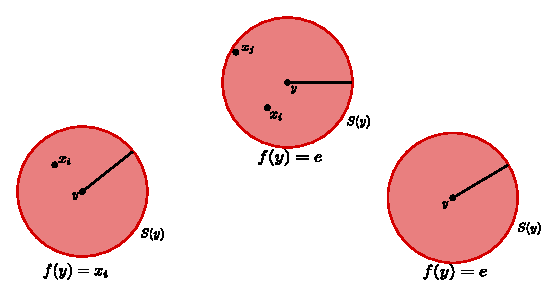
\includegraphics[scale=1]{Figures/Chapter3/decoding_spheres.eps}
        \caption{The Decoding spheres of the code $\Cc$.}
        \label{fig_3.2}
    \end{figure}
    For any $y \in A_Y^n$, if  $S(y)$ contains exactly one such codeword of
    $\Cc$,  $x_i$, then  $f(y)=x_i$. Otherwise, $f(y)=e$, an error. That is, if
    there are no codewords, or more than one (disctinct) codeword in any given
    sphere, we introduce an error.

    Now, transmitting $x_i$ and recieving $y$, error can occure if, and only if
    either $x_i \notin S(y)$, or $x_i,x_j \in S(y)$ for $i \neq j$ and $x_i$ and
    $x_j$ distinct. Thus, we get:
    \begin{equation*}
        P_e^{(i)}=P(x_i \in S(y))+\sum_{j=1, j \neq i}^M{P(x_j \in S(y))}
    \end{equation*}
    Define then the indicator functions $\Delta$ and  $\Delta'$ of  $T'$ as:
    \begin{equation*}
        \Delta(x,y)=\begin{cases}
                    1,  &   (x,y) \in T'        \\
                    0,  &   (x,y) \notin T'     \\
               \end{cases}
    \end{equation*}
    and
    \begin{equation*}
        \Delta'(x,y)=\begin{cases}
                    0,  &   (x,y) \in T'        \\
                    1,  &   (x,y) \notin T'     \\
                \end{cases}
    \end{equation*}
    Then $P_e^{(i)} \leq \sum{\Delta'(x_i,y)p(y|x_i)}+\sum_{j \neq
    i}\sum_{y}{\Delta(x_j,y)p(y|x_i)}=Q_i(x_1, \dots, x_M)$ (note, $Q_i$ is not
    the transition matrix  $Q$).

    Now, define the probability distribution on $A_X^n$ b y:
    \begin{equation*}
        P(x_1, \dots, x_M)=\prod_{i=1}^M{p(x_i)}
    \end{equation*}
    This distribution corresponds to picking a code $\Cc$ at randomby picking
    its codewords independently according to the probability distribution $p(x)$
    achieving $C(\beta_0)$. Then viewing $Q_i(x_1, \dots, x_M)$ as a random
    variable on $A_X^n$, we find :
    \begin{equation*}
        E(Q_i(x_1, \dots, x_M))=E_1+\sum_{j=1}^M{E_2^{(j)}}
    \end{equation*}
    Now,
    $E_1=\sum{\prod_{i=1}^M{p(x_i)}}\sum{\Delta'(x_i,
    y)p(y|x_i)}=\sum{p(x_i)p(y|x_i)\Delta'(x_i,y)}=\sum{p(x,y)\Delta'(x,y)}=
    P((x,y) \notin T') \leq P((x,y) \notin T)+P(x \notin B)$. Thus:
    \begin{equation*}
        E_1 \leq P(I(x,y)<nR')+P(b(x)>\beta n)
    \end{equation*}
    Notice, however that $I(x,y)=\sum{I(x_k,y_k)}$ which has mean $C(\beta_0)$;
    and since $R'<C(\beta_0)$, by the weak law of large numbers:
    \begin{equation*}
        \lim_{n \rightarrow \infty}{P(I(x,y)<nR')}=0
    \end{equation*}
    So, $E_1 \rightarrow_0$ as $n \rightarrow \infty$. Similarly,
    $P(b(x)<\beta n) \rightarrow 0$ as $n \rightarrow \infty$.

    On the otherhand,
    $E_2^{(j)}=\sum_{i=1}^M{\prod{p(x_i)}}\sum{\Delta(x_j,y)p(y|x_j)}=
    \sum{p(x_j)\Delta(x_j,y)}\sum{p(x_i)p(y|x_i)}=\sum{p(x_j)\Delta(x_j,y)p(y)}$.
    So
    \begin{equation*}
        E_2^{(j)} \leq \sum_{(x,y) \in T}{p(x)p(y)}
    \end{equation*}
    Now, $p(x)p(y) \leq p(x,y)2^{-R'n}$, thus $E_2^{(j)} \leq 2^{-R'n}$, so we
    get:
    \begin{equation*}
        E(Q_i) \leq P(I(x,y)<nR')+P(b(x)>\beta n)+M_2^{-R'n}
    \end{equation*}
    So $E(Q_i) \leq M_2^{-R'n}$ as $n \rightarrow \infty$. If
    $M=2^{\ceil{Rn}+1}$, then $E(Q_i) \leq 2^{-n(R'-R)+2}$; and since $R'>R$, we
    get  $E(Q_i) \rightarrow 0$ as $n \rightarrow \infty$. Therefore, for $n$
    large enough, and  $M=2^{\ceil{Rn}+1}$, we get:
    \begin{equation*}
        E(Q_i)<\frac{\epsilon}{2}
    \end{equation*}
    For $\epsilon>0$ small enough, and we have established condition $(2)$ of
    the theorem.

    Now define:
    \begin{equation*}
        P_e(x_1, \dots, x_M)=\frac{1}{M}\sum_{i}^M{P_e^{(i)}(x_1, \dots, x_M)}
    \end{equation*}
    to be the overall error probability assuming each codeword of the code $\Cc$
    is transmitted with probability $\frac{1}{M}$. Regardign
    $P_e(x_1, \dots, x_M)$ as a random variable over $A_X^n$, we have for  $n$
    large, and  $M=2^{\ceil{Rn}+1}$. that $E(P_e)<\frac{\epsilon}{2}$. Thus
    there is a code for which $P_e(x_1, \dots, x_M)<\frac{\epsilon}{2}$, and
    consequently for which:
    \begin{equation*}
        P_e^{(i)}<\frac{\epsilon}{2}<\epsilon
    \end{equation*}
    For $\epsilon>0$ small enough.

    Now, it may be that the code $\Cc$ contains codewords $x_i$ for which
    $b(x_i)> \beta n$, or $P_E^{(i)} \geq \epsilon$, or both; furthermore, if
    more than half the codewords have $P_e^{(i)} \geq \epsilon$, then
    $P_e>\frac{\epsilon}{2}$, which cannot happen. So deleting all the codewords
    $x_i$ for which $P_e^{(i)} \geq \epsilon$ from $\Cc$, we get a code  $\Cc'$
    with  $|\Cc'|=2^{\ceil{Rn}}$ codewords for which $P_e^{(i)}<\epsilon$.
    Notice, then that if $b(x_i)>\beta n$ for some $x_i \in \Cc'$, then  $x_i
    \notin S(y)$, making $P_e^{(i)}=1>\epsilon$. So $\Cc'$ cannot contain non
    $\beta$-admissible codewords, and we complete the proof.
\end{proof}
\begin{remark}
    The proof of the channel coding theorem is very involved and warrants closer
    study of the arguments to better understand.
\end{remark}
\begin{corollary}[The Channel Coding Theorem for Discrete Memoryless Channels.]
    For any $R<C_{\max}$ and $\epsilon>0$, there exists a code  $\Cc=\{x_1,
    \dots, x_M\}$ of length $n$ and decoding rule such that:
    \begin{enumerate}
        \item[(1)] $M \geq 2^{\ceil{Rn}}$....

        \item[(2)] $P_e^{(i)}<\epsilon$ for all $1 \leq i \leq M$.
    \end{enumerate}
\end{corollary}
\begin{proof}
    Let $\beta_0=\beta_{\max}$.
\end{proof}
